%\documentclass[twocolumn,10pt]{article}
%\usepackage{hyperref}

\documentclass[applications]{gen-bioinformatics}

\makeatletter
\renewcommand\boldmath{\@nomath\boldmath\mathversioo
n{bold}}
\makeatother

\usepackage{amssymb,amsfonts,url,times}
\usepackage{graphics}
\usepackage{amsmath}
\usepackage{dcolumn}
\newcolumntype{.}{D{.}{.}{-1}}
%\usepackage{hlight}

\urlstyle{rm}
\def\email#1{#1}



\newcommand{\Rfunction}[1]{{\texttt{#1}}}
\newcommand{\Robject}[1]{{\texttt{#1}}}
\newcommand{\Rpackage}[1]{{\textit{#1}}}
\newcommand{\Rmethod}[1]{{\texttt{#1}}}
\newcommand{\Rfunarg}[1]{{\texttt{#1}}}
\newcommand{\Rclass}[1]{{\textit{#1}}}
\providecommand{\OO}[1]{\operatorname{O}\left(#1\right)}
 

\author[1]{\pfnm{Shweta}
  \pinit{}
  \psnm{Gopaulakrishnan}}

\author[1]{\pfnm{Samuela}
  \pinit{}
  \psnm{Pollack}}

\author[1]{\pfnm{Benjamin}
  \pinit{}
  \psnm{Stubbs}}

\author[2]{\pfnm{Herv\'e}
  \pinit{}
  \psnm{Pag\`es}}

\author[3]{\pfnm{John}
  \pinit{}
  \psnm{Readey}}

\author[4]{\pfnm{Sean}
  \pinit{}
  \psnm{Davis}}

\author[5]{\pfnm{Levi}
  \pinit{}
  \psnm{Waldron}}

\author[6]{\pfnm{Martin}
  \pinit{T}
  \psnm{Morgan}}

\author[1]{\pfnm{Vincent}
  \pinit{J}
  \psnm{Carey}}

\address[1]{\porgdiv{Channing Division of Network Medicine}
  \porgname{Brigham and Women's Hospital}
  \pstreet{181 Longwood Avenue }
  \pcity{Boston}
  \postcode{02115}
  \pcnty{USA}}

\address[2]{\porgdiv{Systems Bioinformatics}
  \porgname{Fred Hutchinson Cancer Research Center}
  \pstreet{Fairview Avenue }
  \pcity{Seattle}
  \postcode{}
  \pcnty{USA}}

\address[3]{
  \porgname{HDF Group}
  \pstreet{}
  \pcity{Seattle}
  \postcode{}
  \pcnty{USA}}

\address[4]{\porgdiv{Center for Cancer Research}
  \porgname{NCI}
  \pcity{Bethesda}
  \pcnty{USA}}


\address[5]{
  \porgdiv{Institute for Implementation Science in Population Health}
  \porgname{CUNY School of Public Health}
  \pcity{NY}
  \pcnty{USA}}

\address[6]{
  \porgname{RPCI}
  \pstreet{}
  \pcity{Buffalo}
  \postcode{}
  \pcnty{USA}}

 

\begin{document}


\title{restfulSE: a semantically rich interface for cloud-scale genomics
with Bioconductor}
\maketitle

\begin{abstract}
\begin{subabstract}[Summary]
Bioconductor's \verb+SummarizedExperiment+ class unites numerical
assay quantifications with sample- and experiment-level metadata.  
It is the standard Bioconductor class for assays that
produce matrix-like data, used by over 200 packages, but
previously did not support remote data stores.
We describe a deployment of this data model, the 
\verb+restfulSE+ package, for data resources that are
accessible from remote resources via REST APIs.  We illustrate
\verb+SummarizedExperiment+s with remote HDF5 and Google
BigQuery back ends.
\end{subabstract}
\begin{subabstract}[Availability] Package \Rpackage{restfulSE} of Bioconductor
 (\url {www.bioconductor.org}). Open source.
\end{subabstract}
\begin{subabstract}[Contact]reshg@channing.harvard.edu
\end{subabstract}
%\begin{subabstract}[keywords] REST API, HDF5, Bioconductor
\end{abstract}
\section*{Introduction}

The analysis of multiomic archives like The Cancer Genome Atlas (TCGA, \url{https://cancergenome.nih.gov/})
and single-cell transcriptomic experiments such as the 10x 1.3 million
mouse neuron dataset (\url{https://support.10xgenomics.com/single-cell-gene-expression/datasets}) typically begin with downloads of large files and
conversion of file contents into formats based on local preferences.
In this paper we consider how targeted queries of large remote genomic
data resources can be conducted using methods available for
Bioconductor's \verb+SummarizedExperiment+ class.  This approach can
be used to centralize large data archives, diminish redundant disk
consumption, and facilitate ad hoc and interactive analysis of data
subsets without downloading entire datasets. Clients for
HDF5 (\url{https://www.hdfgroup.org/}) or BigQuery (\url{https://cloud.google.com/bigquery/}) are available in numerous languages; our
Bioconductor interface permits access to remote archives of genomic
data with familiar and semantically meaningful programmatic idioms,
while abstracting the remote interface from end users
and developers.

\section*{Description}

\subsection*{The SummarizedExperiment class and related methods}

Let $Q$ denote a matrix of quantifications arising from a genome
scale assay with $G$ assay features measured on $N$ experimental
samples.  The elements of $Q$ are the numbers $q_{ij}, i = 1, \ldots, G,
j = 1, \ldots, N$.  In the 10x mouse neuron dataset, $G=27998$ and $N=1.3$ million.
When these quantifications are managed in a Bioconductor \verb+SummarizedExperiment X+, the matrix $Q$ is programmatically bound to a $G \times F$
table of feature-level metadata (e.g., gene or transcript names and
characteristics) accessible by the \verb+rowData+ method, and to an $N \times R$ table of sample-level metadata accessible by \verb+colData+ \citep{Huber2015}. 
The standard subsetting idiom \verb+X[G,S]+ expresses filtering of 
the all the information in $Q$ and the associated metadata
to features \verb+G+ and samples \verb+S+.  A \verb+GRanges+ 
instance \citep{Lawrence2013} defining genomic coordinates for features may be bound to \verb+X+,
facilitating queries defined by genomic location (using, for example, \verb+subsetByOverlaps+) to isolate features
coincident with or near the elements of a set of query genomic ranges (eg., binding peaks).  This outline of genomic data representation
and analysis is characteristic of Bioconductor.

\subsection*{Managing quantifications remotely}

\noindent
\textbf{Google BigQuery.} The Institute for Systems Biology Cancer
Genomics Cloud project (ISB-CGC) \citep{ISBCGC} uses 
Google BigQuery to provide access to
various public cancer genomics resources including
TCGA and the PanCancer Atlas \citep{Hoadley2018}.
The \verb+pancan_SE+
function of \Rpackage{restfulSE} constructs queries that derive
SummarizedExperiment instances using quantifications and annotations
for PanCancer atlas experiments
managed in BigQuery tables.  

\noindent
\textbf{HDF Cloud.}
An AWS S3-based distributed data object model for
HDF5 datasets, including a
RESTful API to structure, populate, and query HDF5 archives,  has been implemented by the HDF Group. The authors have constructed and
made publicly available a
number of datasets of interest in genome science for this framework.

\noindent
\textbf{DelayedArray.}
The \Rpackage{restfulSE} package provides interfaces to 
BigQuery and HDF Cloud so that 
the numerical content housed in these services
satisfies the Bioconductor \verb+DelayedArray+ API \citep{Pages2018}.  
%Any \verb+DelayedArray+ instance can serve as the \verb+assay+
%component of a \verb+SummarizedExperiment+ instance.  Thus the
%capacities of \verb+SummarizedExperiment+ to bind semantically
%rich metadata to genome-scale assays are extended implicitly to
%data resources for which no standards exist for
%associating substantive metadata.  
In conjunction with the \Rpackage{rhdf5client} and \Rpackage{bigrquery} packages,
\Rpackage{restfulSE} translates filtering and selection operations
which are readily defined using \verb+rowData+, \verb+rowRanges+,
and \verb+colData+ into formal queries resolvable by the HDF5 and
BigQuery services.  Numerical results are transmitted from
server to client only when needed.

\section*{Results}

The RESTful \verb+SummarizedExperiment+ representation
allows complicated research queries to be obtained in a concise,
fast, convenient and robust fashion, as illustrated by
the following examples.

\textbf{BigQuery back end.} Figure \ref{pancanPanel} illustrates the 
use of the \Rpackage{restfulSE} protocol
with the ISB-CGC BigQuery back end.  In Figure 5C
of \citet{Bailey2018}, it is suggested that
microsatellite instability (MSI) is associated with
different expression signatures of immune cell infiltration
for adenocarcinomas of colon (COAD) and stomach (STAD), and
uterine corpus endometrial carcinoma (UCEC).  Bailey's
detailed quantifications of microsatellite instability
are not available; a categorization of MSI was
obtained from the \Rpackage{curatedTCGAData} system \citep{Ramos2017}.
Code at the top of Figure \ref{pancanPanel} employs
functions in the \Rpackage{BiocOncoTK} package that build on
restfulSE functionality to a) authenticate the
user to the BigQuery platform, b) select a tumor
type (COAD) and assay for SummarizedExperiment
construction, c) bind MSI available values as
sample-level data variable \verb+msiTest+, d)
acquire and transform the PD-L1 
(Entrez ID 29126)
expression values, and e) form the stratified boxplot. 
The basic findings of Bailey et al. are replicated.
Enhancement of the code to produce the 3 x 3 tableau
is demonstrated in the \Rpackage{BiocOncoTK} vignette.
Note that in this example, expression values are
only downloaded for a single gene, without altering
the end user programming paradigm.

\noindent
\textbf{HDF Cloud back end.}  Figure \ref{hdffig}
demonstrates construction of a RESTful SummarizedExperiment
for expression data on 1.3 million neurons.
The syntax \verb+tenx[,s]+ generates a delayed selection for
all genes with samples 
identified in vector \verb+s+.  Invoking the \verb+assay()+
method triggers RESTful queries to the object store at \verb+URL_hsds()+.
These can be serviced in parallel, with
throughput dependent on the configuration
of the HSDS server and its load at time of request.
Replies can be requested in JSON or binary formats;
\Rpackage{rhdf5client} utilities handle parsing the
responses into R matrix structures.
In this example, data for only four of 1.3 million neurons
are downloaded and used to compute sums of RNA-seq read
counts.  The \verb+DelayedArray+ framework leveraged here
enables basic computations of this kind without loading the
entire matrix into memory.

\section*{Performance}

We focus on pursuit of reliability,
expressivity, and scalability using \Rpackage{restfulSE}.  
\textit{Reliability:} 
The \Rpackage{restfulSE}, \Rpackage{rhdf5client},
and \Rpackage{BiocOncoTK} packages are accompanied by detailed unit
tests that compare retrievals to known values.  In the
case of BigQuery table queries, the test
suite composes random queries 
in both BigQuery SQL and in the SummarizedExperiment idiom.  Results
are tested for concordance.  \textit{Expressivity:} The code
segments in Figures \ref{pancanPanel} and \ref{hdffig} are
complex but easy to break down.  The joining and
reshaping of pancan-atlas tables in BigQuery corresponding
to the code in Figure \ref{pancanPanel}
can be checked through the query history in the BigQuery
interface.  The acquisition of expression values required
five nested SELECT statements; the query for assay quantifications
was 6000 characters in length.
The R code is 223 characters including comments.
\textit{Scalability.}  BigQuery is intrinsically auto-scaling,
but charges accrue with the amount of data scanned, 
so query design can have effects on throughput
and cost.  We rely on the \Rpackage{bigrquery} and \Rpackage{dbplyr} packages for
efficient translation of R-oriented data manipulations to 
BigQuery SQL.  Throughput with HDF Cloud 
is dependent upon the configuration of the object server,
the relationship of numerical data layout to prevalent access
patterns, and the degree to which queries capitalize on
API efficiencies like chunk-based retrieval.  For both
back ends, proper design and deployment of the querying client can
lead to throughput that scale with client-side resources.

\section*{Conclusions}

Cloud-scale storage and retrieval strategies are of significant
interest for genome science.  The \Rclass{SummarizedExperiment} class
unifies assay data with substantive sample- and experiment-level
metadata, and its API for managing and interrogating
genome-scale experiment archives is used in numerous
analytic packages.  The \Rpackage{restfulSE} package exposes high-performance
cloud-resident data stores to users and
algorithms as \verb+SummarizedExperiment+s.  Continued improvements
in efficiency of
representation and query resolution for assay data and metadata
will help to achieve the potential of a federated data ecosystem for
enhanced discovery in biology through interactive genome-scale analysis.



\begin{figure}[bb]
\begin{verbatim}
library(BiocOncoTK) # uses restfulSE
bq = pancan_BQ() # need CGC_BILLING
seCOAD = bindMSI(buildPancanSE(bq, 
  acronym="COAD", assay="RNASeqv2"))
boxplot(split(log2(as.numeric(assay(
 seCOAD["29126",]))+1), seCOAD$msiTest))
\end{verbatim}
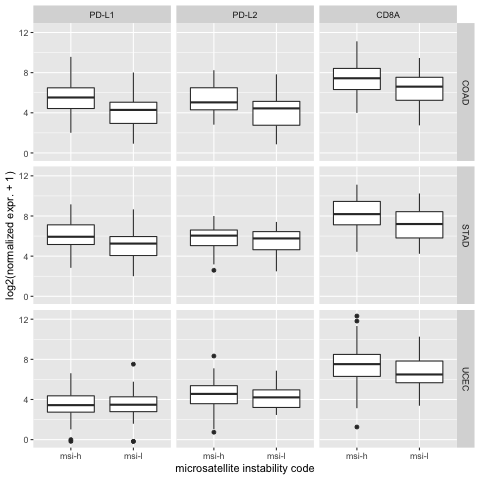
\includegraphics[height=8.0cm]{imm3x3.png}
\caption{Top: Code for base graphics display of boxplot
corresponding to top left panel of lower display.
Bottom: Reassessment of immune infiltrate expression
patterns stratified by microsatellite instability
status and tumor type, as reported in \cite{Bailey2018}.
The vignette for package BiocOncoTK includes all
code needed to produce the nine panel display.}
\label{pancanPanel}
\end{figure}

\begin{figure}[bb]
\begin{verbatim}
eh = ExperimentHub::ExperimentHub()
tenx = eh[["EH554"]]
library(rhdf5client)
tenxA = HSDS_Matrix(URL_hsds(), 
     "/home/reshg/tenx_full.h5") 
assays(tenx) = SimpleList(counts=tenxA)
library(DelayedMatrixStats)
colSums(assay(tenx[,1:4]))
\end{verbatim}
\caption{Code to construct a RESTful SummarizedExperiment
for the 10x Genomics 1.3 million neuron RNA-seq quantifications.
URL\_hsds() returns a string with 
the URL for HDF Kita Lab.  The results are
4046, 2087, 4654, and 3193.}
\label{hdffig}
\end{figure}

\section*{Acknowledgments}
Support for the development of this software was provided by NIH grants
U01 CA214846 (Carey, PI) and U24 CA180996 (Morgan, PI).

\bibliography{BioC}

\end{document}
